\chapter{Results}
\label{results}
In this Chapter are presented the results of our approach in every part of our work. We are going to describe through examples what we have achieved in the motion part, in the communication part, in the coordination part and finally and the most important the overall results which is the real competitive soccer matches against other teams who have participated in one or more RoboCup competitions in the past.

\section{Movement}
This section presents the improvements we have done in the part of agents movements and motions. In general, as we described above in motion Chapter, motion files are generated by other teams or other platforms such as FIIT project or Webots Simulator. The only thing that we could have done is to try improving these motion files until we reached an adequate result for our team. Table~\ref{MotionImprovements} shows the improvements made in motions only in cases that it was possible. 

Optimized walk motion has reached a speed up to .45m/s which is comparable but much slower than the UT Austin Villa's walking engine which produces a walk motion of .71m/s. Furthermore strong kick movement has reached a 5.5 meters range in just 2.5 seconds of execution. Turn motion is using Webots motion files. Turning which has reached to a speed up to 30 degrees per second. 

\begin{table}
\begin{center}
\begin{footnotesize}
\begin{tabular}{ccccc}
\textbf{Motion Version} & \textbf{Walk(m/s)}	& \textbf{Turn(d/s)}	& \textbf{Kick(m (Sec.) )}&\textbf{Strong Kick(m (Sec.) )} \\
\midrule
Webots (Text-Based) 		& 0.11 				& 21 				& 3 				& - \\
FIIT (XML)				& 0.22 				& 25 				& 3 (4) 		& 4 (5) \\
\textbf{AST\_3D} 		& 0.45 	& 30 		& 3 (2.5)& 5.5 (2.5) \\
\end{tabular}
\end{footnotesize}
\end{center}
\label{MotionImprovements}
\caption{Motion's Performance Improvement (Averaged Speeds and Ranges)}
\end{table}



\section{Communication}
Testing communication process through ideal external communication, when only our team has the ability to send messages accomplishes good results. Agents were able to ``hear'' all their teammates in an averaged 24 simulation cycles. In addition, even in competition's situations when both teams had the ability to send messages to their teammates the results remained approximately the same. Table~\ref{CommunicationResults} presents the communication phases' performance during communication process. We can realize that there are not serious delays in these communication phases. This happens due to the fact soccer simulation server does not allow players to send messages in the same server cycle. We take advantage of the fact that there are separately tracked capacities for both teams, because teams should not be able to block the hear perceptors of their opponents by shouting permanently. In fact, we send  messages every three cycles, so, it does not a restriction for our team, and server allows us to shout messages in most cases.

\begin{table}[h!]
\begin{center}
\begin{footnotesize}
    \begin{tabular}{ccc}
    \textbf{Communication Phase} 	& \textbf{Ideal (Cycles (Sec.))}			& \textbf{During Match (Cycles (Sec.))} \\
    \midrule
    Init Messages 					& 24  ( 0.48 ) 			& 24 	( 0.48 )		\\
    Coordination Messages			& 24  ( 0.48 )			& 42.5  ( 0.85 )		\\
    Action Messages 				    & 24  ( 0.48 )			& 24 ( 0.48 )	 		\\
    \end{tabular}
    \end{footnotesize}
\end{center}
\label{CommunicationResults}
\caption{Communication Results in Ideal and Match Conditions}
\end{table}



\section{Goalkeeper}
Goalkeeper's behavior was tested against the best team in Robocup 3D Simulation League, UT Austin Villa. To determine his ability to stop opponents from scoring we first do not use a goalkeeper allowing opponent agents to reach our goal and score. Next, we use the goalkeeper but with an ``empty'' behavior with which he was not able to perform any movement or track the ball, standing useless at the center of our goal. Opponent team managed to score seven goals in this occasion equal amount of goal with (No Goalkeeper) test. However, when goalkeeper made use of his current developed behavior he achieved to reduce conceded goal from seven to three. Table~\ref{GoalKeeperResults} presents these results.



\begin{table}[h!]
\begin{center}
\begin{footnotesize}
    \begin{tabular}{cc}
    \textbf{GoalKeeper Type} 	& \textbf{Goals Conceded}\\
    \midrule
    No Goalkeeper						& 7\\
    Goalkeeper, ``Empty'' Behavior	& 7\\
    Goalkeeper, ``Full'' Behavior	& 3\\
    \end{tabular}
    \end{footnotesize}
\end{center}

\label{GoalKeeperResults}
\caption{Goalkeeper Averaged Results in Half-Games.}
\end{table}


\section{Coordination Beliefs Update}

\section{Coordination}
The most significant part of our project. In this section we are going to present the results of the team coordination procedure. As we have discussed during Chapter 5, coordination is responsible for assigning roles to the players, finding strategic positions, computing optimized mappings among players and positions. We have discussed every aspect of this procedure and now it is time to present the results. During test-games, we have tested our software and especially the coordination algorithm which was our major concern. The main characteristics of the team coordination are:

\begin{description}
\item[Attacking Positioning]
Finding and assigning worthy positions to the agents while our team was in an offensive situation was a main goal of our positioning system. In every occasion in which an agent of our team has the ball in its possession, active subset's agents should be assigned worthy positions to support the on ball player. Figure~\ref{fig:AttackingPositioning1} presents an example of this positioning system. As we can realize, active players are given routes to follow to be close to the opponents' goal, seeking to exploit any arising opportunity. Figure~\ref{fig:AttackingPositioning2} presents another example, a possible shoot by the on ball player will give active agents the chance to score a goal.


\begin{figure}[t!]
\centering
  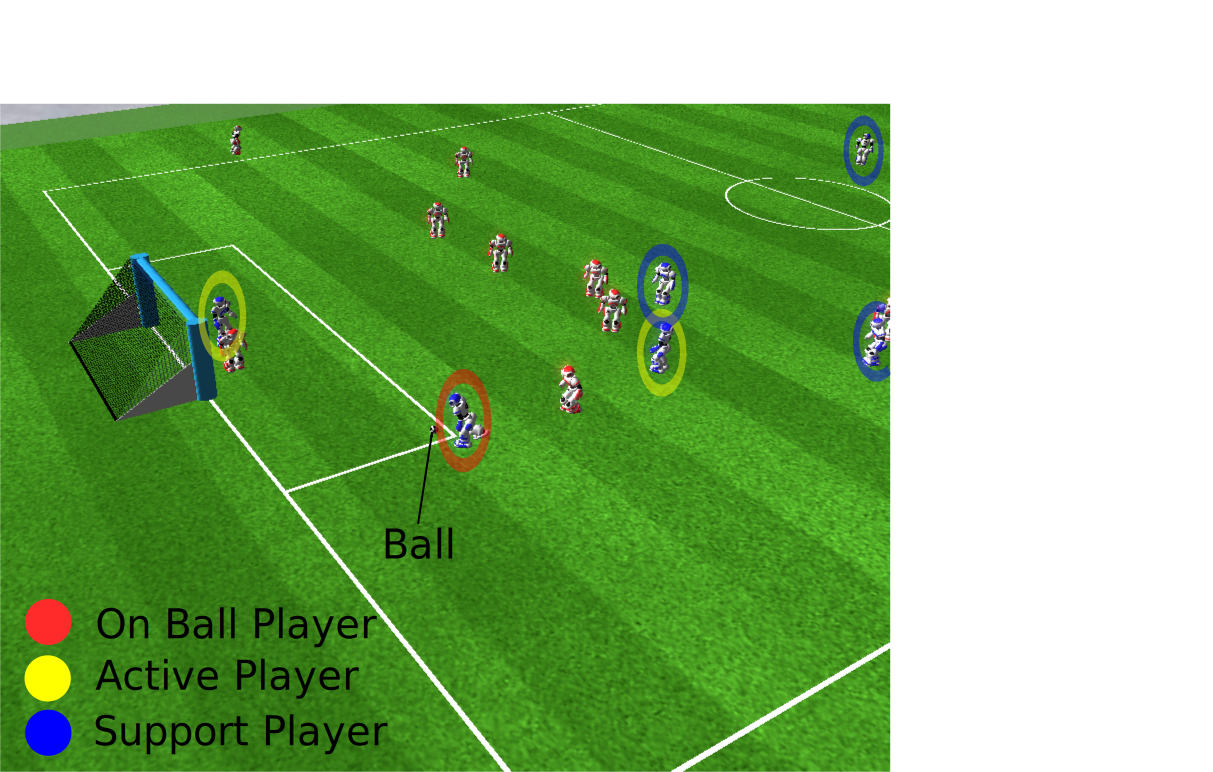
\includegraphics[width=0.8\textwidth]{Chapter5/figures/3.pdf}
  \caption{Attacking Positioning Resulting by Coordination Process, Example 1.} 
  \label{fig:AttackingPositioning1}
\end{figure}

\begin{figure}[t!]
\centering
  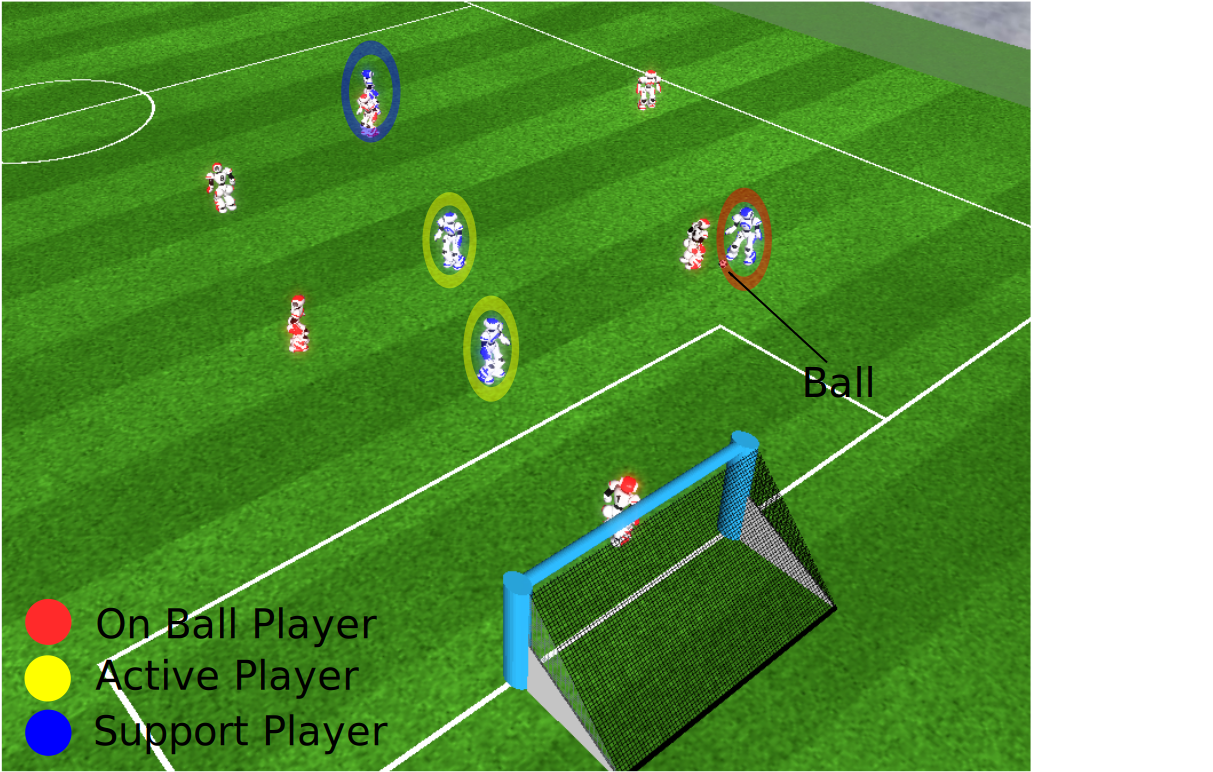
\includegraphics[width=0.8\textwidth]{Chapter5/figures/5.pdf}
  \caption{Attacking Positioning Resulting by Coordination Process, Example 2.} 
  \label{fig:AttackingPositioning2}
\end{figure}


\item[Defensive Positioning]
Finding and assigning useful positions to the agents while our team was in a defensive situation was another main point of our positioning system. In every occasion, in which our team is on a defensive role into the field located in our half, active subset's agents should be assigned worthy positions to support the on ball player and protect possible opponents' routes towards our goal. Figure~\ref{fig:DefendingPositioning} presents an example of this positioning system. As we can realize, active players are given locations to go to be disastrous to a possible opponents' walk to our goal, seeking to clear the ball on any arising opportunity. Figure~\ref{fig:DefendingPositioning1} presents another example, a possible shoot by the on ball player will give active agents the chance to score a goal.


\begin{figure}[t!]
\centering
  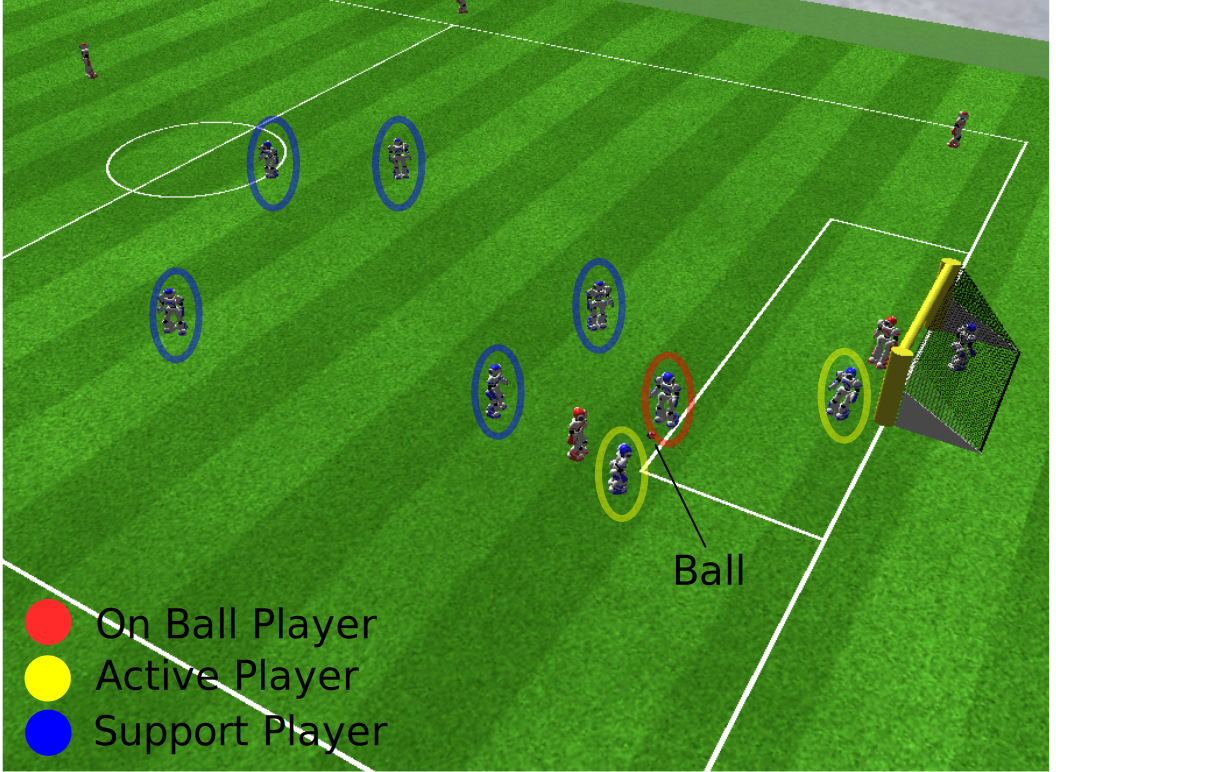
\includegraphics[width=0.8\textwidth]{Chapter5/figures/1.pdf}
  \caption{Defending Positioning Resulting by Coordination Process, Example 1.} 
  \label{fig:DefendingPositioning}
\end{figure}


\begin{figure}[t!]
\centering
  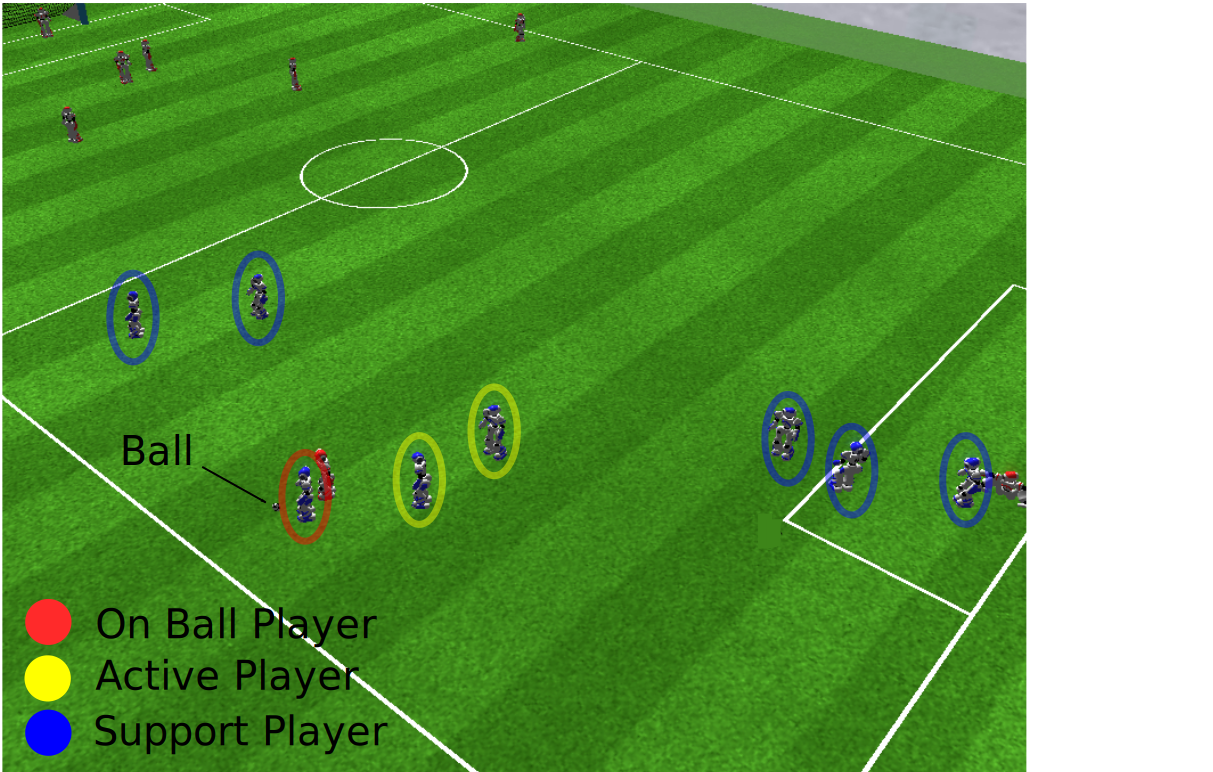
\includegraphics[width=0.8\textwidth]{Chapter5/figures/2.pdf}
  \caption{Defending Positioning Resulting by Coordination Process, Example 2.} 
  \label{fig:DefendingPositioning1}
\end{figure}

\item[Strategic Consistency]
Dynamic role assignment was one of the most significant parts of our team coordination system. In many occasions during game-play we have seen too many times agents changing roles and duties with each other. Team coordination system was built for that, to be adaptable in different situations inside a mostly dynamic environment like robotic soccer. This function resulting our team to have an adequate role distribution in every moment within a simulation soccer game. Agents are assigned a role which will be proven to be worthy and costless in terms of the overall movement of our team into the soccer field. Figure~\ref{fig:StrategicPositioning} presents how this characteristic of the coordination process presents into the field during game time. Active agents as well as on ball player are assigned some roles. Other roles are available to be assigned to other players. Each one of the agents in blue circle is assigned a specific role which is described.

\begin{figure}[t!]
\centering
  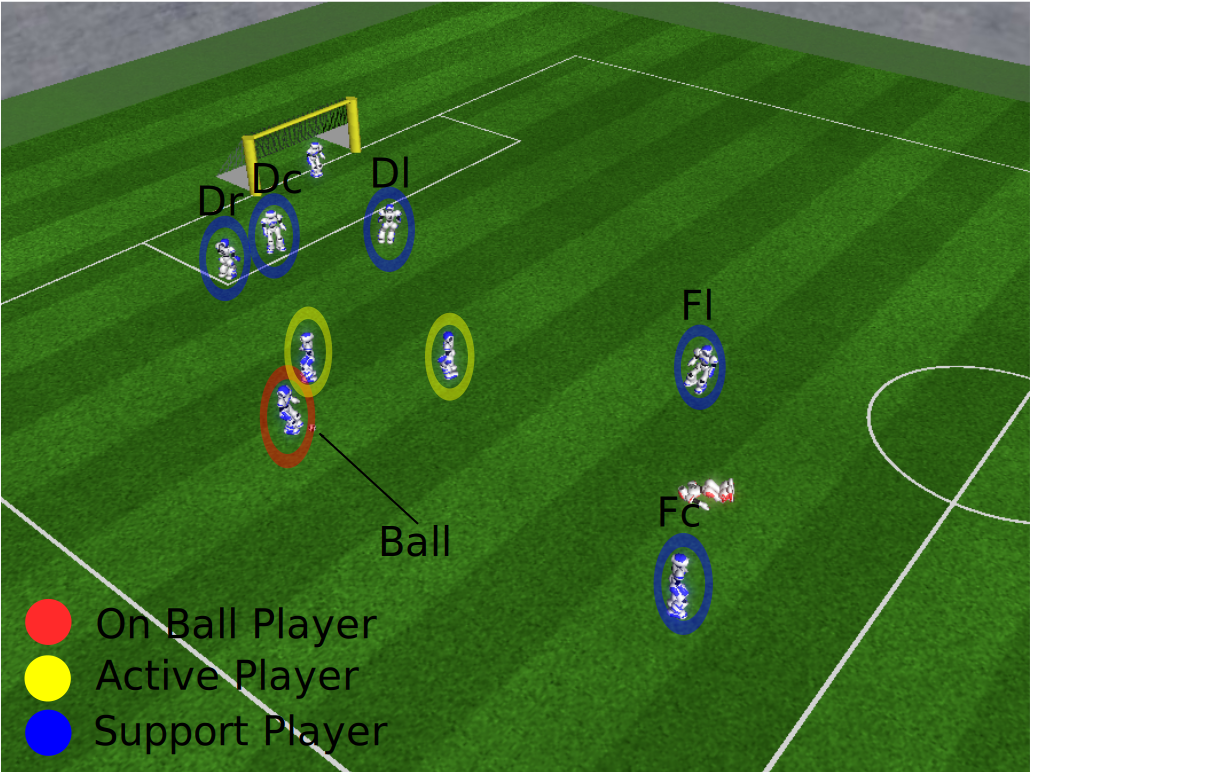
\includegraphics[width=0.8\textwidth]{Chapter5/figures/4.pdf}
  \caption{Strategic Consistency Resulting by Coordination Process Via Team Roles Assignment.} 
  \label{fig:StrategicPositioning}
\end{figure}

\end{description}


\section{Overall Results}
In order to test our software in the most realistic way. We decided to test our team in real conditions playing against teams that have already participated in robocup soccer simulation competitions. Most of these teams have been participating in this competition for more than one years and consist of more than one team members. We have selected nine teams from Instabul's competition and one team (MAK) from Iran open 2011. These teams are:
\begin{description}
\item[RoboCanes]	University of Miami, USA 
\item[UT Austin Villa]	University of Texas at Austin, USA
\item[NomoFC]	Osaka University, Japan
\item[OxBlue]	University of Oxford, UK
\item[L3MSIM]	Paris8 University,France
\item[Kaveh] 	Shahid Rajaee University, Iran University of Science and Technology, Iran
\item[beeStanbul]	Istanbul Technical University, Turkey
\item[Farzanegan]	Farzanegan high school, Iran
\item[MAK]	Ehsan Mosavi, University Of Kerman Mehravaran ,3D Robotics, Iran
\item[FUTK3D]	Fukui University of Technology, Japan
\end{description}

\subsubsection*{Overall Game Results}

\begin{table}[t!]
\begin{center}
    \begin{tabular}{cccccc}
    \textbf{Team} 	& \textbf{W} & \textbf{D} & \textbf{L} & \textbf{AGD}\footnotemark 	& \textbf{Games}   \\
    \midrule
    UTAustinVilla 	& 0		& 0		& 4		& -5.2		& 4 			\\
    Robocanes 		& 0		& 0		& 1		& -6.0		& 1 			\\
    BeeStanbul		& 0		& 0		& 3		& -4.0		& 3				\\
    NomoFC 			& 1		& 2		& 0		& +0.3 		& 3 			\\
    Rail 			& 0		& 4		& 0		& 0.0 		& 4 			\\
    OxBlue 			& 0		& 0		& 2		& -1.5 		& 2 			\\
    FUTK3D 			& 0		& 5		& 0		& 0.0 		& 5 			\\
    FARZANEGAN 		& 1		& 1		& 0		& +0.5 		& 2 			\\
    MAK 		    & 2		& 0		& 0		& +2.0 		& 2 			\\
    L3M-SIM			& 3		& 2   	& 0		& +0.6 		& 5 			\\     
    \end{tabular}
\end{center}
\label{GameResults}
\caption{Full-Game Results}
\end{table}
\footnotetext[1]{AGD: Averaged Goal Difference}


Playing against these teams, most of these have participated into one or more Robocup competitions, we have gained a lot of experience and we have seen how our team reacts in different situations in such a dynamic environment. Due to lack of dynamic motions, our agents has poor movement especially in comparison with the RoboCup Simulation league's best teams. However, we were able to perform well and score some goals against weaker teams of this competition. Better movement will give us exactly what we need in order to be competitive towards the best teams of the league. Judging by the results, I am absolutely sure that we could compete in equal terms with other teams for a position in simulation 3D league either in an open competition or in Robocup itself.

After all these test-matches against teams who have participated into one or more Robocup competitions, we have gained a lot of experience and we have seen how our team reacts in different situations in such a dynamic environment. Due to lack of dynamic motions, our agents has poor movement especially in comparison with the RoboCup Simulation league's best teams. However, we were able to perform well and score some goals against weaker teams of this competition. Better movement will give us exactly what we need in order to be competitive towards the best teams of the league. Judging by the results, I am absolutely sure that we could compete in equal terms with other teams for a position in simulation 3D league either in an open competition or in Robocup itself.

All executable binaries from teams are from \href{http://simspark.sourceforge.net/binaries/RoboCup2011/}{SimSpark Wiki - Previous Events Binaries}. All games had 10 minutes duration, same as real competition matches in official Robocup competition. Server and monitor were running in the same machine\footnotemark. Each team binary was running in a separate machine\footnotemark . Table~\ref{GameResults} presents the results between our and opponent teams. There is information about the goal difference and the number of wins, draws, loses, and the number of test-games.
\footnotetext[1]{\textbf{Server}: Intel Core 2 Duo 3.16 Ghz, 5.8GiB Ram}
\footnotetext[2]{\textbf{Client1}: Intel Core 2 Duo 1.86 Ghz, 2GiB Ram}
\footnotetext[2]{\textbf{Client2}: Intel Quad Core i5 3.3 Ghz,4GiB Ram}


\subsubsection*{Mini Tournament}

Finally, we held a mini tournament in which teams participated in it were selected in order to have a competitive and in equal terms competition. Table~\ref{EasyTournament} presents the result table of this tournament. Win: 3 points, draw: 1 points, loss: 0 points.

\begin{table}[t!]
\begin{center}
\begin{tabular}{l*{6}{c}r}
Team              	& P & W & D & L & F  & A & Pts \\ \hline
\textbf{AST3D} 		& \textbf{8} & \textbf{2} & \textbf{6} & \textbf{0} & \textbf{ 2} & \textbf{0} &  \textbf{12}  \\
NomoFC            	& 2 & 0 & 1 & 1 &  0 & 1 &  1  \\
L3M-SIM     		& 2 & 0 & 1 & 1 &  0 & 1 &  1  \\
Rail     		    & 2 & 0 & 2 & 0 &  0 & 0 &  2  \\
farzanegan     		& 2 & 0 & 2 & 0 &  0 & 0 &  2  \\
\end{tabular}
\end{center}
\label{EasyTournament}
\caption{Mini Tournament}
\end{table}






